% =========================================================
% CONFIGURACION DEL DOCUMENTO
% =========================================================
\providecommand{\main}{..}
\documentclass[../main.tex]{subfiles}

% =========================================================
% CONTENIDO
% =========================================================
\begin{document}		
\chapter{Estado del arte}
\label{cha:02_estado_del_arte}

	\begin{figure}[H]
		\centering
		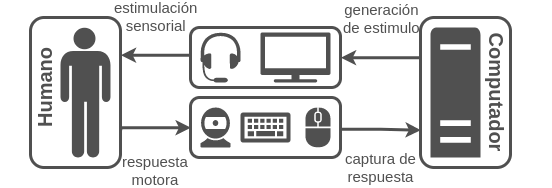
\includegraphics[width=0.8\textwidth]{cap_02_diagram}
		\caption{Diagrama general de la interfaz hombre-máquina.}
		\label{fig:02_diagrama_interfaz}
	\end{figure}

	\begin{figure}[H]
		\centering
		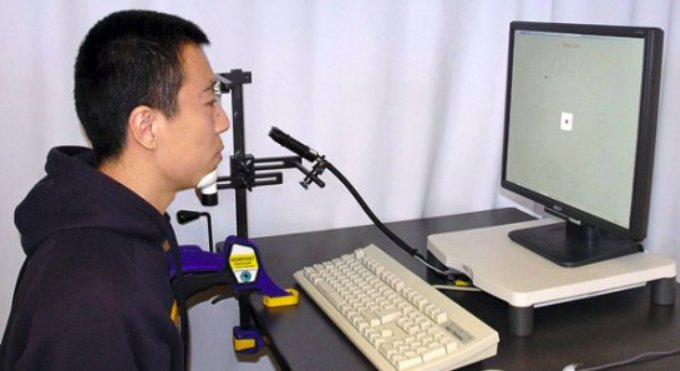
\includegraphics[width=0.5\textwidth]{cap_02_setup}
		\caption{Ejemplo de \gls{setup} experimental \cite{website:baseInfo}.}
		\label{fig:02_ejemplo_setup}
	\end{figure}

	\section{Sistemas de seguimiento ocular}
	\label{sec:02_sistemas_de_seguimiento_ocular}
		\subsection{Movimiento ocular}
		\label{sub:02_movimiento_ocular}


		\subsection{Métodos de captura}
		\label{sub:02_metodos_de_captura}
			\subsubsection{Un poco de historia}
			\label{ssub:02_un_poco_de_historia_tracker}

			\subsubsection{Tecnologías actuales}
			\label{ssub:02_tecnologias_actuales}
				\begin{enumerate}
					\item \textbf{De contacto directo}

					\item \textbf{Seguimiento ocular}

					\item \textbf{Medición de potencial eléctrico}

				\end{enumerate}

			\subsubsection{Comparativa}
			\label{ssub:02_comparativa_eyetracker}
			
		\subsection{Sistemas comerciales más relevantes}
		\label{sub:02_sistemas_comerciales_más_relevantes}
			\begin{enumerate}
				\item \textbf{EyeGaze}

				\item \textbf{EyeLink}

				\item \textbf{EyeTribe}

				\item \textbf{IViewX}

				\item \textbf{Tobii}

			\end{enumerate}

	\section{Sistemas de estimulación visual}
	\label{sec:02_sistemas_de_estimulacion_visual}
		\subsection{Hardware de estimulación}
		\label{sub:02_hardware_de_estimulacion}
			\subsubsection{Un poco de historia} 
			\label{ssub:02_un_poco_de_historia_monitores}

			A lo largo de la historia las tecnologías utilizadas 

			\subsubsection{Tecnologías actuales} 
			\label{ssub:02_tecnologías_actuales}
				\begin{enumerate}
					\item \textbf{Monitores CRT}

					\item \textbf{Monitores LED, oLED, LCD}

				\end{enumerate}

			\subsubsection{Comparativa}
			\label{ssub:02_comparativa_monitores}
			
		\subsection{Software de estimulación}
		\label{sub:02_software_de_estimulacion}
			\subsubsection{Software más relevante}
			\label{ssub:02_software_mas_relevante}
				\begin{enumerate}
					\item \textbf{PsychoPy}

					\item \textbf{PsychoToolbox}

					\item \textbf{VissionEgg}

					\item \textbf{Presentation}

				\end{enumerate}

			\subsubsection{Comparativa}
			\label{ssub:02_comparativa_software}

		\subsection{Experimentos de estimulación}
		\label{sub:02_experimentos_de_estimulacion}

\end{document}
